% Lecture Template for ME3001-001-Tristan Hill - Spring 2017 - Fall 2017
% 
% Mechanical Engineering Analysis with MATLAB
%
% Introduction to Analysis

% Document settings
\documentclass[11pt]{article}
\usepackage[margin=1in]{geometry}
\usepackage[pdftex]{graphicx}
\usepackage{multirow}
\usepackage{setspace}
\usepackage{hyperref}
\usepackage{color,soul}
\usepackage{fancyvrb}
\usepackage{framed}
\usepackage{wasysym}
\usepackage{multicol}

\pagestyle{plain}
\setlength\parindent{0pt}
\hypersetup{
    bookmarks=true,         % show bookmarks bar?
    unicode=false,          % non-Latin characters in Acrobat’s bookmarks
    pdftoolbar=true,        % show Acrobat’s toolbar?
    pdfmenubar=true,        % show Acrobat’s menu?
    pdffitwindow=false,     % window fit to page when opened
    pdfstartview={FitH},    % fits the width of the page to the window
    pdftitle={My title},    % title
    pdfauthor={Author},     % author
    pdfsubject={Subject},   % subject of the document
    pdfcreator={Creator},   % creator of the document
    pdfproducer={Producer}, % producer of the document
    pdfkeywords={keyword1} {key2} {key3}, % list of keywords
    pdfnewwindow=true,      % links in new window
    colorlinks=true,       % false: boxed links; true: colored links
    linkcolor=red,          % color of internal links (change box color with linkbordercolor)
    citecolor=green,        % color of links to bibliography
    filecolor=magenta,      % color of file links
    urlcolor=blue           % color of external links
}

% assignment number 
\newcommand{\NUM}{1 } 
\newcommand{\VSpaceSize}{2mm} 
\newcommand{\HSpaceSize}{2mm} 

\definecolor{mygray}{rgb}{.6, .6, .6}

\setulcolor{red} 
\setstcolor{green} 
\sethlcolor{mygray} 

\begin{document}

\textbf{ \LARGE ME 3001 Lecture - Introduction to Analysis} \vspace{3mm}\\
\textbf{ \hspace*{5mm}Tristan W. Hill - Tennessee Technological University - Spring 2020 } \vspace{3mm}\\

\begin{itemize}


	\item \textbf{ \LARGE What is analysis? What is this class about?}\\
			
			\Large{``detailed examination of the elements or structure of something, typically as a basis for discussion or interpretation."}  \vspace{10mm} \\ 



		\item \textbf{ \LARGE How does it apply to mechanical engineering?}\\

			\Large{``mathematical modeling of engineering systems and the theoretical and numerical solutions to non-linear equations, systems of linear equations, and ordinary and partial differential equations''}\\
			
			\Large{``mathematical methods for solving mechanical engineering problems with modern computing tools''} \vspace{5mm}\\

		\item \textbf{ \LARGE What areas of engineering will we cover?}\\
		
		\begin{itemize}
		
			\item Statics and Mechanics\\
			\item Rigid Body Dynamics\\
			\item Fluid Dynamics\\
			\item Thermodynamics and Heat Transfer\\
			\item Vibrations\\
		
		\end{itemize}
		\newpage
		
		\item \textbf{ \LARGE We will be doing some mathematics in this class!}\\
		\begin{multicols}{2}
		\begin{itemize}
		
			\item Algebra and Arithmetic\\
			\item Matrix\slash Linear Algebra \\
			\item Calculus \\
			\item Ordinary and Partial \\Differential Equations \\
			\item The Fourier Series \\
			
		
		\end{itemize}
		\end{multicols}
				
		\item \textbf{ \LARGE This class is different than a traditional mathematics class.}\\ 
				\begin{itemize}
					\item By nature engineering problems are hard to solve on paper.\\
					
					\item So, will be using calculators but we will also be using...\\
									
					\item \hspace{1mm} \vspace{10mm}\\
									
				\end{itemize}
				
		\item \textbf{ \LARGE Modern Computing Tools}\\ 		
		
				\begin{itemize}
					\item  \hspace{1mm} \vspace{5mm}\\
					
					\item  \hspace{1mm} \vspace{5mm}\\
					
					\item  \hspace{1mm} \vspace{5mm}\\
									
				\end{itemize}
	\newpage
	
	\item \textbf{ \LARGE Main Topics to be Covered}\\\\ 
	\Large{ Mathematical Modeling of Engineering Problems Involving: }\\
		\begin{enumerate}
			\item Solutions to Non-Linear Equations \vspace{5mm}\\
				\begin{itemize}
					\item Rigid Body Dynamics \\\\
					
					\item Optimization and Design \\
					
				\end{itemize}
			
			\item Solving Systems Linear Equations \vspace{5mm}\\
				\begin{multicols}{2}
				\begin{itemize}
					\item Statics and Structural  \\
					
					\item Equilibrium Equations\\
					
					\item The Eigenvalue Problem\\
					
					\item Mechanisms and Machines\\
					
				\end{itemize}
				\end{multicols}
			\item Ordinary Differential Equations \vspace{5mm}\\
				\begin{multicols}{2}
				\begin{itemize}
					\item Rigid Body Dynamics\\
					\item Thermodynamics and Heat Transfer\\
					\item Electronics and Circuits\\
				\end{itemize}
				\end{multicols}
			\item Partial Differential Equations \vspace{5mm}\\
				\begin{itemize}
					\item Fluid Dynamics\\
					\item Thermodynamics and Heat Transfer\\
				\end{itemize}
		\end{enumerate}
	\end{itemize}
	\LARGE
	\begin{enumerate}	
		
		\item \textbf{  Solutions to Non-Linear Equations}\\\\ 
			\begin{itemize}
					\item What is a non-linear equation? \vspace{20mm} \\
					\item What does it mean to solve a non-linear equation? \vspace{20mm} \\
					\item Standard form of this problem:\\\\
					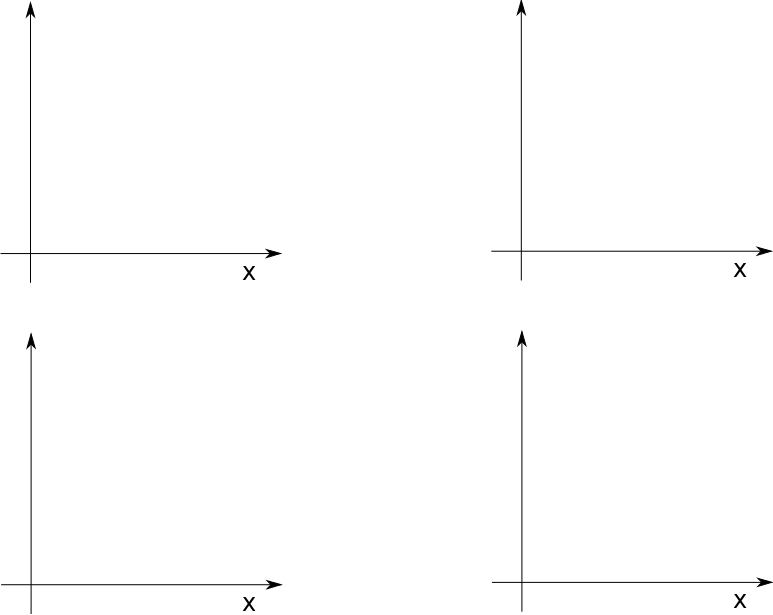
\includegraphics[scale=.5]{lecture1_fig1.png}
			\end{itemize}
\newpage			
			\item \textbf{  Solving Systems Linear Equations}\\\\ 
			\begin{itemize}
					\item What is a system of linear equations?\vspace{20mm} \\
					\item What does it mean to solve a  system of linear equations? \vspace{20mm} \\
					\item A very simple example:\\\\
					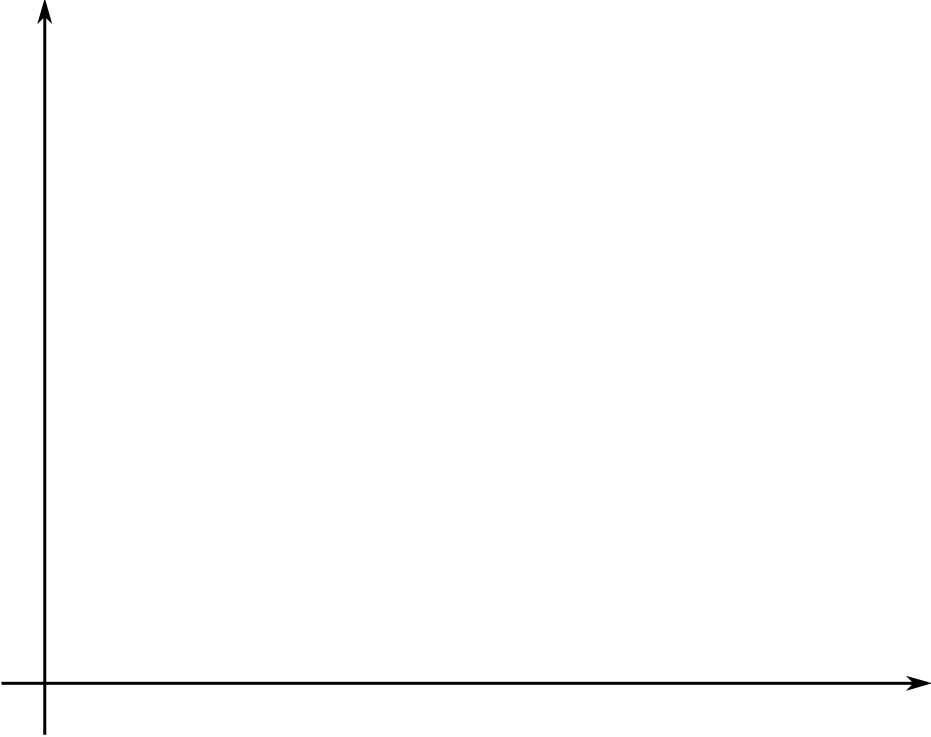
\includegraphics[scale=.45]{lecture1_fig2.png}
			\end{itemize}
			
			\item \textbf{  Ordinary Differential Equations}\\\\ 
			\begin{itemize}
					\item What is a Differential Equations? What about a system of them?\vspace{20mm} \\
					\item What does it mean to solve a differential equation? \vspace{20mm} \\
					\item A very simple example:\\\\
					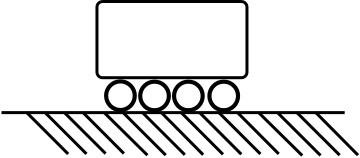
\includegraphics[scale=.6]{lecture1_fig3.png}\\\\
					\Large {ODE:}\vspace{30mm}\\
					\Large {Solution:}\\\\
			\end{itemize}
\newpage			
			\item \textbf{  Partial Differential Equations}\\\\ 
			\begin{itemize}
					\item What is different about a Partial Differential Equation? \vspace{20mm} \\
					
					\item What is different about the solution to a PDE?  \vspace{20mm}  \\
					
					\item What does this allow us to do? \\
					
			\end{itemize}
	\end{enumerate}
		



	

\end{document}



